\chapter{Algorithmes et Analyse}




\section{Descripteurs}
Pour pouvoir appliquer notre mesure de similarité entre deux images et calculer les poids de nos particules, on a besoin de pouvoir extraire de l'information de nos images. Ainsi allons nous utiliser des descripteurs. \\
Un descripteur est un morceau d'information extrait d'une image sous forme de vecteur. Il permettra de reconnaitre un motif ou une structure spécifique au cours de notre vidéo. Pour calculer un descripteur on s'appuie sur l'information bas niveau de nos images (valeur des pixels, contours, gradients, ...).

\subsection{Histogramme de gradient orienté}

Nous utiliserons en particulier les histogrammes de gradients orientés (HOG) qui sont des descripteurs proposés par Navneet DALAL et Bill TRIGGS \cite{dalal_histograms_2005}. Ils correspondent à la distribution de l'orientation des contours locaux d'une image. \\

Les HOG sont calculés par DALAL et TRIGGS ainsi : \\

Une première étape de pré-traitement de l'image afin de normaliser les couleurs et d'appliquer une correction gamma à celle-ci puis la convertir en niveau de gris. Ici la normalisation du HOG est suffisante et cette étape est donc facultative, on s'est contenté de la conversion en niveau de gris. \\

L'étape suivante est le calcul de la carte des gradients en x et en y qui correspondent respectivement à la variation horizontale et verticale des gradients. On effectue une convolution centrée sur le pixel cible. Parmi les différents filtres possibles, les masques que nous utilisons sont $[-1, 0, 1]$ pour les gradients en x et $[-1, 0, 1]^{T}$ pour les gradients en y, aussi appelés filtres de Sobel. Ces masques se sont révélés plus performants dans la littérature \cite{dalal_histograms_2005}.\\

À partir de ces deux cartes de gradients on pourrait calculer la carte des modules des gradients. Néanmoins, afin d'augmenter l'efficacité du descripteur, le HOG n'est pas directement calculé à partir de l'image.\\

En effet l'image est divisée en "cellules", elles-mêmes regroupées en "blocs". On choisit des cellules de 6*6 pixels et des blocs de 3*3 cellules.\\

Pour chaque bloc, on calcule le HOG de chaque cellule. Le HOG du bloc correspond à la concaténation du HOG des cellules le composant. Pour une meilleure invariance face à l'illumination et à l'ombrage on effectue une normalisation du HOG du bloc (norme euclidiennne). Pour un vecteur x, on a :

\[ \sum_{k=0}^{n} (x_{k})^{2} \]

Donc le HOG de l'image est la concaténation de l'ensemble des HOG de chacun de ses blocs.

\begin{figure}[!htbp]
\center
	\subfloat{{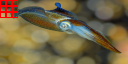
\includegraphics[height=3cm]{Squid_colors_2resized.png}}}
\caption{Bloc d'un HOG.}
\label{fig:cuttlefish_bloccells}
\end{figure}

Les histogrammes sont construits grâce aux mesures des angles des gradients et à leurs intensités. De la même manière qu'avec la taille des blocs et des cellules, on doit choisir la structure de notre histogramme. Étant donné que nous travaillons sur des angles, nous choisirons un histogramme à neuf classes et nous utiliserons des angles non signés (compris entre $[0; 180°]$).
Ainsi pour un pixel $p(x,y)$ l'angle est défini par :

\[ angle_{p} = |\arctan (\grad y, \grad x)*\frac{180}{\pi}| \]

De même que son intensité par :

\[ intensite_{p} = \sqrt{\grad x^{2} + \grad y^{2}} \]

Pour chaque pixel, on répartit son intensité proportionnellement dans les deux classes les plus proches de l'angle qui lui est associé. 
Par exemple, prenons $\grad x = 10$ et $\grad y = 10$ on obtient une intensité d'environ $14.14$ et un angle de $45°$. De cette manière la classe centrée en $40$ recevra les trois quarts ($1 - |\frac{5}{20}|$)et la classe centrée en $60$ recevra le quart restant($1 - |\frac{15}{20}|$) de l'intensité.\\

% Note : prendre gradx = grady = sqrt(2) est plus stylé mais je sais pas si c'est sage

Enfin pour affiner notre descripteur nous effectuerons le déplacement du bloc suivant :

\[ \frac{T_{cellule} * T_{bloc}}{2} \]

$T_{cellule}$ est la taille en pixels de la cellule,
$T_{bloc}$ est la taille en nombre de cellules d'un côté du bloc.
Ainsi on a : $\frac{6*3}{2} = 9$, de plus, un bloc faisant plus de 9 pixels de côté, on a un chevauchement des blocs et donc des pixels pris en compte plusieurs fois. Cela permet au vecteur de mieux caractériser l'image cible.

\begin{figure}[!htbp]
\center
	\subfloat{{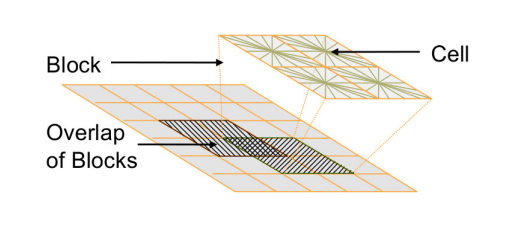
\includegraphics[height=3cm]{blocoverlap.png}}}
\caption{Déplacement d'un bloc.}
\label{fig:blocOverlap}
\end{figure}

\subsection{HOG en cascade}

Pour enrichir notre vecteur caractéristique on peut utiliser HOG en cascade qui combine les HOG de l'image à différentes résolutions. Pour procéder on calcule les HOG sur une succession de sous-régions inclusives et les ajoutons au HOG global, comme décrit dans l'article \cite{qiang_zhu_fast_2006}. De cette manière on ajoute de l'information spatiale à notre descripteur.

\begin{figure}[!htbp]
\center
	\subfloat{{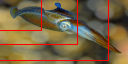
\includegraphics[height=3cm]{Squid_colors_2hogc.png}}}
\caption{HOG en cascade.}
\label{fig:cuttlefish_hog}
\end{figure}




\section{Mesures de similarité}
Après avoir obtenu les vecteurs descripteurs de chaque particule, nous les comparons avec le vecteur descripteur de référence.\\
Pour comparer deux vecteurs descripteur, nous utilisons des mesures de similarité, qui nous indiquerons si les deux vecteurs sont plus ou moins similaire. La mesure de similarité donne 0 si les vecteurs sont exactement similaire, et 1 si ils sont complètement opposés.

\subsection{Distance de Bhattacharyya}
La distance de Bhattacharyya, comme définit dans l'article \cite{bhattacharyya_measure_1960}, permet de calculer une distance entre deux lois de probabilité discrètes. Elle est définie pour deux lois $X$ et $Y$ par la formule:
$$D_{B}(X, Y) = \sqrt{1 - BC(X, Y)}$$
ou bien encore, par la formule:
$$D_{B}(X, Y) = -\ln(BC(X, Y))$$

Où $BC(X, Y)$ est appelé coefficient de Bhattacharyya et est définit par la formule:
$$\sum_{k \in X \hspace{0.1cm} ou \hspace{0.1cm} k \in Y} \sqrt{X(k)*Y(k)}$$


\subsection{Cosine similarity}
La similarité cosinus (Cosine similarity), est une distance, un score, basé sur le cosinus de l'angle entre deux vecteurs.\\
Donc, à partir d'un vecteur descripteur X et du vecteur descripteur de référence Y, nous pouvons calculer le cosinus de l'angle formé par les deux vecteurs, qui est donné par la formule:
$$Sc(X, Y) = \frac{X \cdot Y}{\|X\|\|Y\|}$$\\


\clearpage
\section{Filtre à particule}
Le filtre à particule, aussi connu sous le nom de bootstrap, ou algorithme de condensation, est basé sur une méthode de Monte Carlo, c'est à dire utiliser un ensemble de particule discrète pour représenter la densité de probabilité associé au système que l'on souhaite modéliser. L'idée principale du filtre à particule est d'approcher une distribution, impossible ou difficile à estimer directement, grâce à un ensemble d'échantillons pondérés $S=\{(X_{n}, w_{n})|n=1...N\}$, où $X_{n}$ indique la nième particule, $w_{n}$ indique l'importance de la particule, ou le poids de celle-ci, et $N$ est le nombre total de particule. Plus d'information peuvent être trouvé aux références suivantes \cite{russell_norvig} et \cite{rlabbe}.\\
\\
Cet algorithme a, par exemple, pu être utilisé avec le descripteur HOG, comme dans ces articles \cite{xu_human_2010}, \cite{kong_particle_2019}, \cite{qiang_zhu_fast_2006} et \cite{dalal_histograms_2005}, mais il peut également être utilisé avec d'autre descripteur, ou combinaison de descripteur, comme HOG cascade combiné avec LBP (Local Binary Pattern).\\
\\
Les particules que le filtre utilise peuvent être définies de plusieurs façon, nous avons choisi de définir une particule, comme un point en 2D, la vélocité et l'accélération de ce point, et la demi largeur et demi hauteur de la bounding box délimitant notre cible, mais il est possible de changer cette définition. A un instant $t$, une particule est donc représentée par un vecteur à 8 dimensions:
$$X^{t}=\left[ x^{t}, \dot{x}^{t}, \ddot{x}^{t}, y^{t}, \dot{y}^{t}, \ddot{y}^{t}, l^{t}, h^{t} \right]^{T}$$
Où $(x^{t}, y^{t})^{T}$, $(\dot{x}^{t}, \dot{y}^{t})^{T}$ et $(\ddot{x}^{t}, \ddot{y}^{t})^{T}$ sont les coordonnées, vélocités et accélération du centre de notre cible en pixel, respectivement, $(l^{t}, h^{t})$ décrit la bounding box de notre cible en pixel avec la demi largeur et la demi hauteur.\\
\\
Bien qu'il existe plusieurs variantes de cet algorithme, le principe général reste le même (voir figure \ref{alg:particlefilter_basic}). Il s'agit d'utiliser les particules pour déterminer l'état de notre système à un instant $t$, en faisant une prédiction de nos particules dans le temps puis en ajoutant du bruit, et en combinant cette prédiction avec une observation $z$ (résultats de capteurs, ou images d'une vidéo, par exemple) afin de mettre à jour les poids de chacune des particules. Une fois les poids mis à jour, on vérifie combien de particule participent réellement à l'estimation de l'état de notre système, et si ce nombre est en dessous d'un certain seuil, on effectue une étape de ré-échantillonnage en gardant les particules de poids fort, et en supprimant celles de poids faible. Finalement, on peut estimer l'état de notre système, en prenant la moyenne pondérée de nos particules (MLE, Maximum Likelihood Estimation) ou en prenant comme estimation la particule de poids le plus fort (MAP, Maximum A Posteriori).

\begin{algorithm}
	\caption{Filtre à particule général}\label{alg:particlefilter_basic}
	\KwData{Une observation $z$}
	\KwResult{Une estimation de l'état de notre système}
	\ForEach{Particules p}{
		Prédiction de $p$ grâce à un modèle de prédiction $f$ et $\nu$ du bruit blanc: $\hat{X}_{p}^{t} = f(X_{p}^{t-1}, \nu)$\\
		Traitement de l'observation grâce à un modèle de mesure $h$ et $n$ le bruit de l'observation: $z^{t} = h(z, n)$\\
		Combinaison de $\hat{X}_{p}^{t}$ avec $z^{t}$ pour mettre à jour le poids de $p$: $w_{p}^{t}$
	}
	Normalisation des poids des particules: $$w_{p}^{t} = \frac{w_{p}^{t}}{\sum_{i=0}^{NB_{particule}} w_{i}^{t}}$$
	\If{le nombre de particule effective est inférieur à un certain seuil}{
		Ré-échantillonnage des particules pondérées par leur poids
	}
	Estimation de l'état de notre système:
	$$(MLE) \hspace{0.4cm} X^{t} = \frac{1}{NB_{particule}} * \sum_{p=0}^{NB_{particule}} X_{p}^{t}*w_{p}^{t}$$
	ou
	$$(MAP) \hspace{0.4cm} X^{t} = \underset{p}{\arg\max} \hspace{0.2cm} w_{p}^{t}$$
\end{algorithm}

Dans notre cas, le modèle de mesure sera effectué en calculant la similarité entre un descripteur de référence $F_{ref}$ et les descripteurs de chaque particule. Au préalable, chaque particule ce voit associer un patch de l'image courante qui est récupéré en utilisant la position et la bounding box de la particule, puis en dimensionnant le patch obtenu à une dimension fixée en amont par l'utilisateur.\\
Cette liste de patch est ensuite donnée à une fonction de mesure de similarité, qui, pour chacun des patch, renvoi un coefficient de similarité ($coeff\_sim$).\\
Ces coefficients de similarité sont ensuite utilisés pour calculer le poids de chaque particule, grâce à une distribution gaussienne centrée en 0 et de déviation standard $\sigma$ (dans notre cas $\sigma=n$, le bruit de l'observation):
$$w_{p}^{t} = \frac{1}{\sqrt{2\pi\sigma^{2}}}e^{-\frac{(coeff\_sim_{p})^{2}}{2\sigma^{2}}}$$
Après estimation de l'état de notre système, nous calculons le descripteur associé à cet état et remplaçons le descripteur de référence $F_{ref}$ par celui-ci.\\
\\
Le modèle de prédiction, quant à lui, utilise la méthode des différences finies d'ordre 3, c'est-à-dire que nous considérons les trois derniers états de la particule pour calculer sa position, vélocité et accélération actuelle. Cependant, d'autres modèle auraient pu être choisi, comme le modèle de prédiction utilisant les équations physique du mouvement, qui a aussi été implémenté.\\
La méthode des différences finies est basée sur les formules suivante:
\begin{equation} \label{eq:vel}
\begin{split}
\dot{x}^{t} = \frac{x^{t} - x^{t-1}}{dt}\\
\dot{y}^{t} = \frac{y^{t} - y^{t-1}}{dt}
\end{split}
\end{equation}
\vspace{0.4cm}
\begin{equation} \label{eq:accel}
\begin{split}
\ddot{x}^{t} = \frac{\dot{x}^{t} - \frac{x^{t-1} - x^{t-2}}{dt}}{dt}\\
\ddot{y}^{t} = \frac{\dot{y}^{t} - \frac{y^{t-1} - y^{t-2}}{dt}}{dt}
\end{split}
\end{equation}
\vspace{0.4cm}
\begin{equation} \label{eq:pos}
\begin{split}
x^{t+dt} = \frac{1}{2} \cdot \ddot{x}^{t} \cdot dt^{2} + \dot{x}^{t} \cdot dt + x^{t} + \nu\\
y^{t+dt} = \frac{1}{2} \cdot \ddot{y}^{t} \cdot dt^{2} + \dot{y}^{t} \cdot dt + y^{t} + \nu
\end{split}
\end{equation}

Avec $dt$ l'intervalle de temps entre chaque image de la vidéo, et $\nu$ le bruit gaussien pour la prédiction.\\
\\
Au cours de la vidéo, il arrive que la cible ce rapproche ou s'éloigne de la caméra, si les dimensions de la bounding box sont fixes, on peut perdre en qualité sur le suivi car la bounding box peut inclure trop d'éléments parasites, ou au contraire, n'inclure qu'une petite partie de la cible.\\
Pour palier ce problème, nous effectuons également une prédiction sur les dimensions de la bounding box, définit par les formules suivante, comme définit dans \cite{kong_particle_2019}:
\begin{equation} \label{eq:gamma}
\gamma=
\begin{cases}
\begin{aligned}
	-0.05,& \hspace{0.4cm}		0 \leq p \leq 0.2\\
    -0.0125,& \hspace{0.4cm}	0.2 \le p \leq 0.4\\
    0,& \hspace{0.4cm}			0.4 \le p \leq 0.6\\
    0.0125,& \hspace{0.4cm}		0.6 \le p \leq 0.8\\
    0.05,& \hspace{0.4cm}		0.8 \le p \leq 1
\end{aligned}
\end{cases}
\end{equation}
Où $p$ est un réel aléatoire entre [0,1].\\
On a alors:
\begin{equation} \label{eq:Bbox}
\begin{split}
l^{t} = l^{t-1} * (1+\gamma) + \nu\\
h^{t} = h^{t-1} * (1+\gamma) + \nu
\end{split}
\end{equation}

En assemblant chacune des parties précédentes, on obtient alors l'algorithme final du filtre à particule, dont un example avec une configuration spécifique est donné dans l'algorithme \ref{alg:particlefilter}.


\begin{algorithm}
	\caption{Filtre à particule}\label{alg:particlefilter}
	\KwData{Une vidéo sous-marine de seiche}
	\KwResult{La liste des positions et bounding box de la cible dans la vidéo}
	\ForEach{Images $t$ de la vidéo}{
		\eIf{Première image}{
			Détection de la seiche dans l'image grâce a YOLOv7\\
			Calcul du descripteur de référence : $F_{ref}^{0}$
		}{
			\ForEach{Particules p}{
				Prédiction de la position (équation \ref{eq:pos}) et de la bounding box (équation \ref{eq:Bbox}) de $p$ dans $t$ en fonction de ses états précédents\\
				Calcul du descripteur du patch correspondant à $p$: $F_{p}^{t}$\\
				Calcul du coefficient de similarité entre $F_{p}^{t}$ et $F_{ref}^{t-1}$: $coeff\_sim_{p}^{t}$\\ 
				Calcul du poids de $p$ dans $t$ :
					$$w_{p}^{t} = \frac{1}{\sqrt{2\pi\sigma^{2}}}e^{-\frac{(coeff\_sim_{p}^{t})^{2}}{2\sigma^{2}}}$$
			}
			Ré-échantillonnage des particules pondérées par leurs poids\\
			Estimation de la position et bounding box de la seiche dans $t$:
				$$X^{t}=\frac{1}{NB_{particule}}*\sum_{p=0}^{NB_{particule}} X_{p}^{t}*w_{p}^{t}$$
		}
		Mise à jour du descripteur de référence: $F_{ref}^{t}$
	}
\end{algorithm}


\clearpage
